\begin{news}
{2} %columnes
{Torronada}
{ \noindent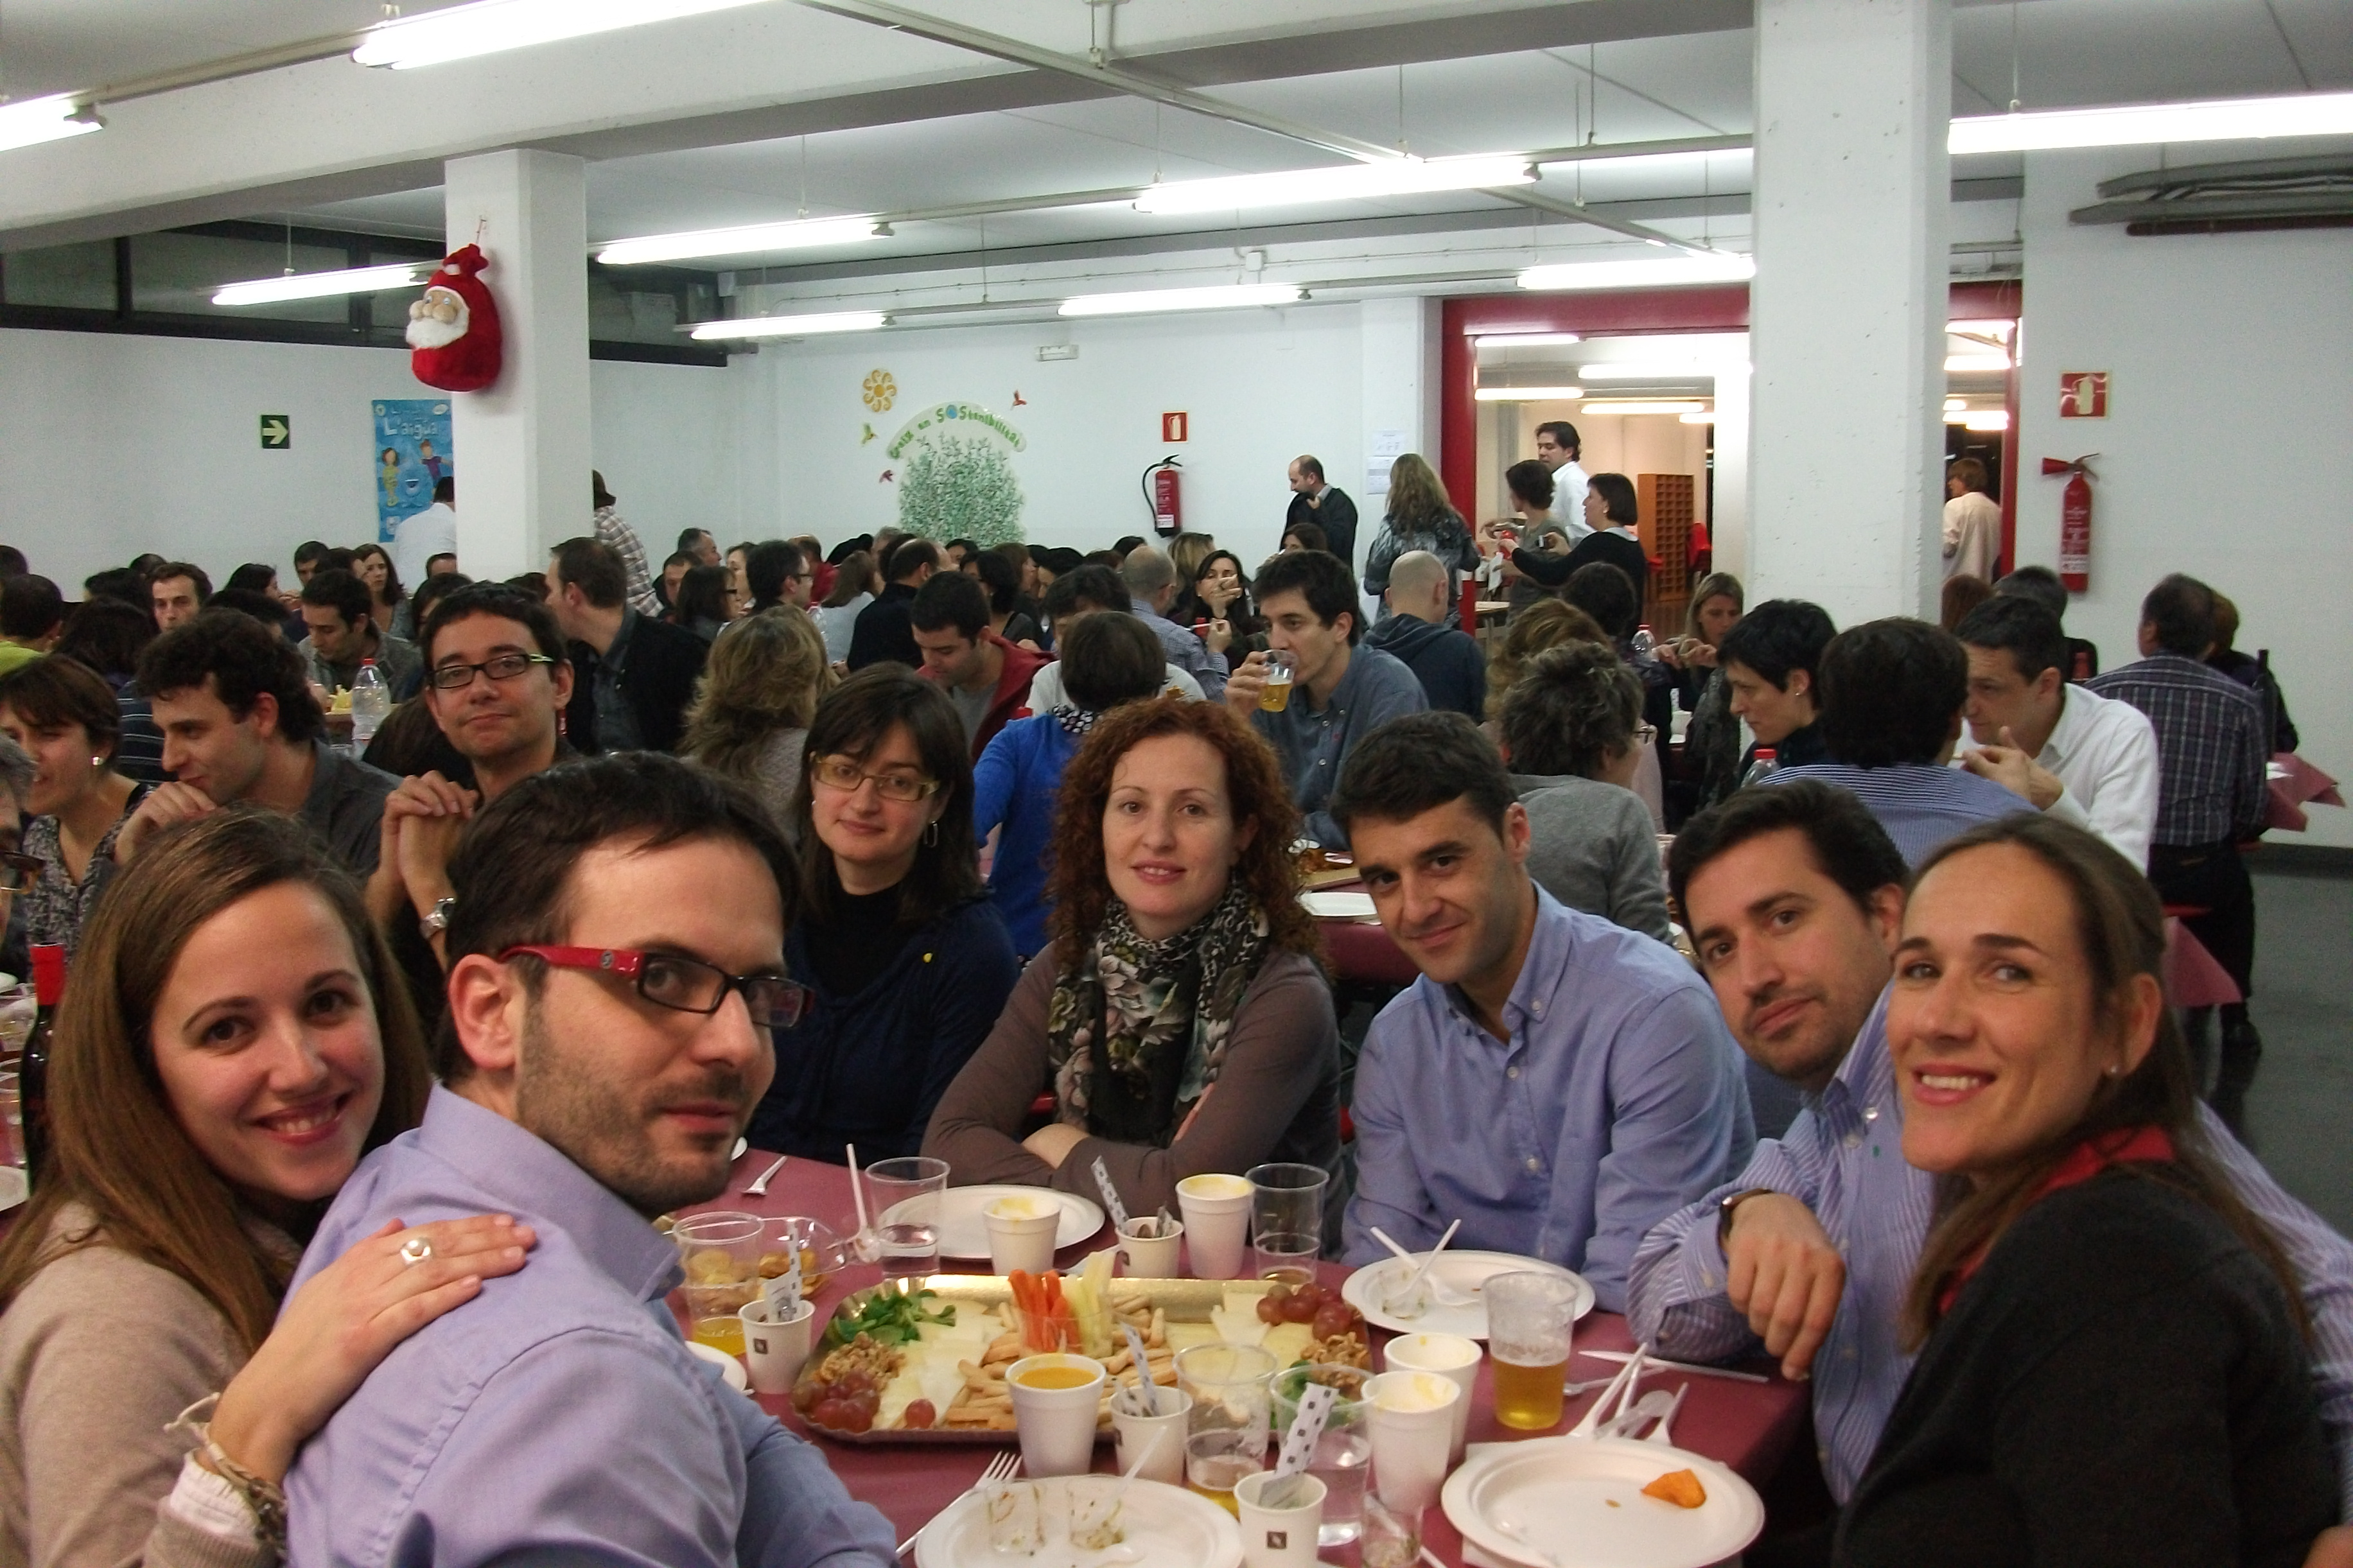
\includegraphics[width=18.2cm,keepaspectratio]{ampa/img/DSCF0909.JPG}}
{Fem Escola}
{0} %pagesof


Un èxit sense precedents, per fi la Torronada va aconseguir reunir a més de 125 mares, pares i mestres de l’escola

El menjador és vesteix de gala, taules amb mantells vermells, plens de viandes, una cadena de pares i mares organitzant les taules, servint el sopar, preparant el cafès i tallant torrons ( en honor al nom de la festa) , no podien faltar.

Aquest any sabíem que la torronada seria diferent, coses per celebrar i molta gent animada s’havia apuntat, això si , ningú sense pandereta, segur que alguna ens tenien preparada, 
6 colors, 6 grups , 6 nadales i 1 guanyador, el grup vermell amb una intervenció magistral i amb la nadala “Los peces en el rio” és va alçar amb el premi, un magnífic Panettone que vam poder gaudir  tots plegats.

I quan acaba el sopar , la tertúlia i el concurs,  comença la marxa … 

\columntitle{lines}{
Cal que els anys no ens treguin la il.lusió.
Això només és el principi!!! 
}

\authorandplace{Text: Gemma López - Fotos: Silvia Serra}{Mares de P5}

\noindent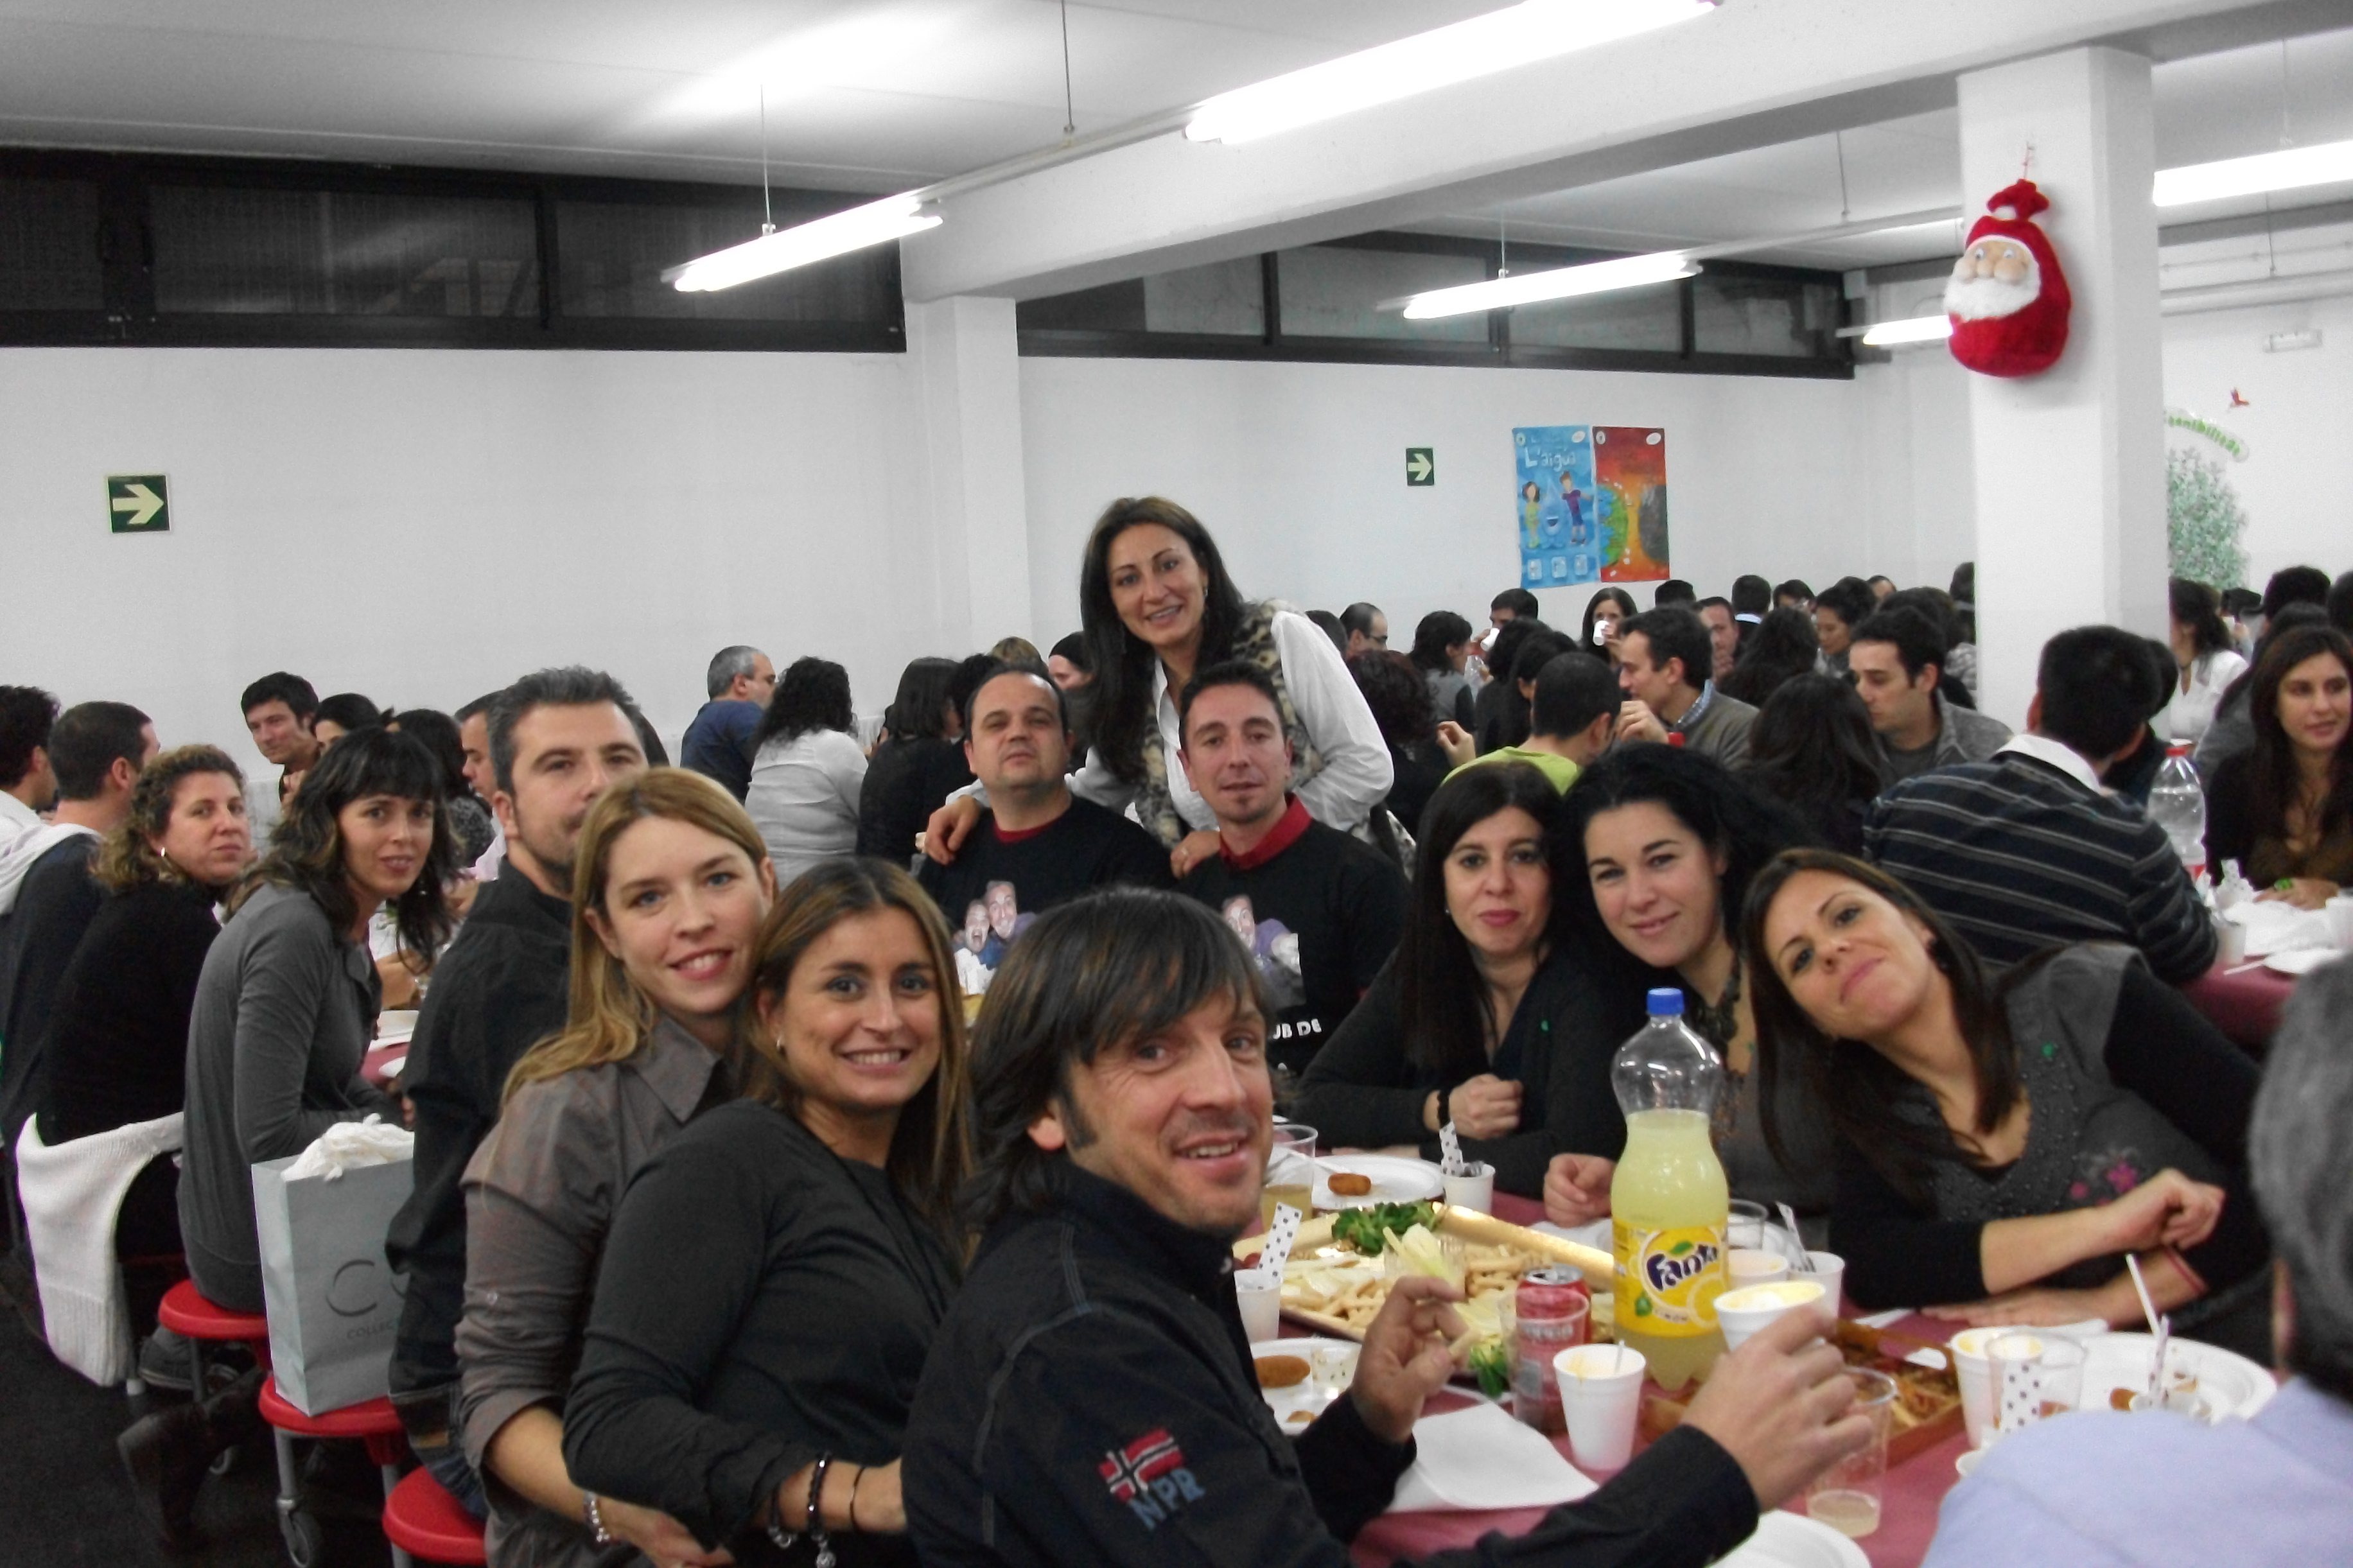
\includegraphics[width=9cm,keepaspectratio]{ampa/img/DSCF0911.JPG}

\noindent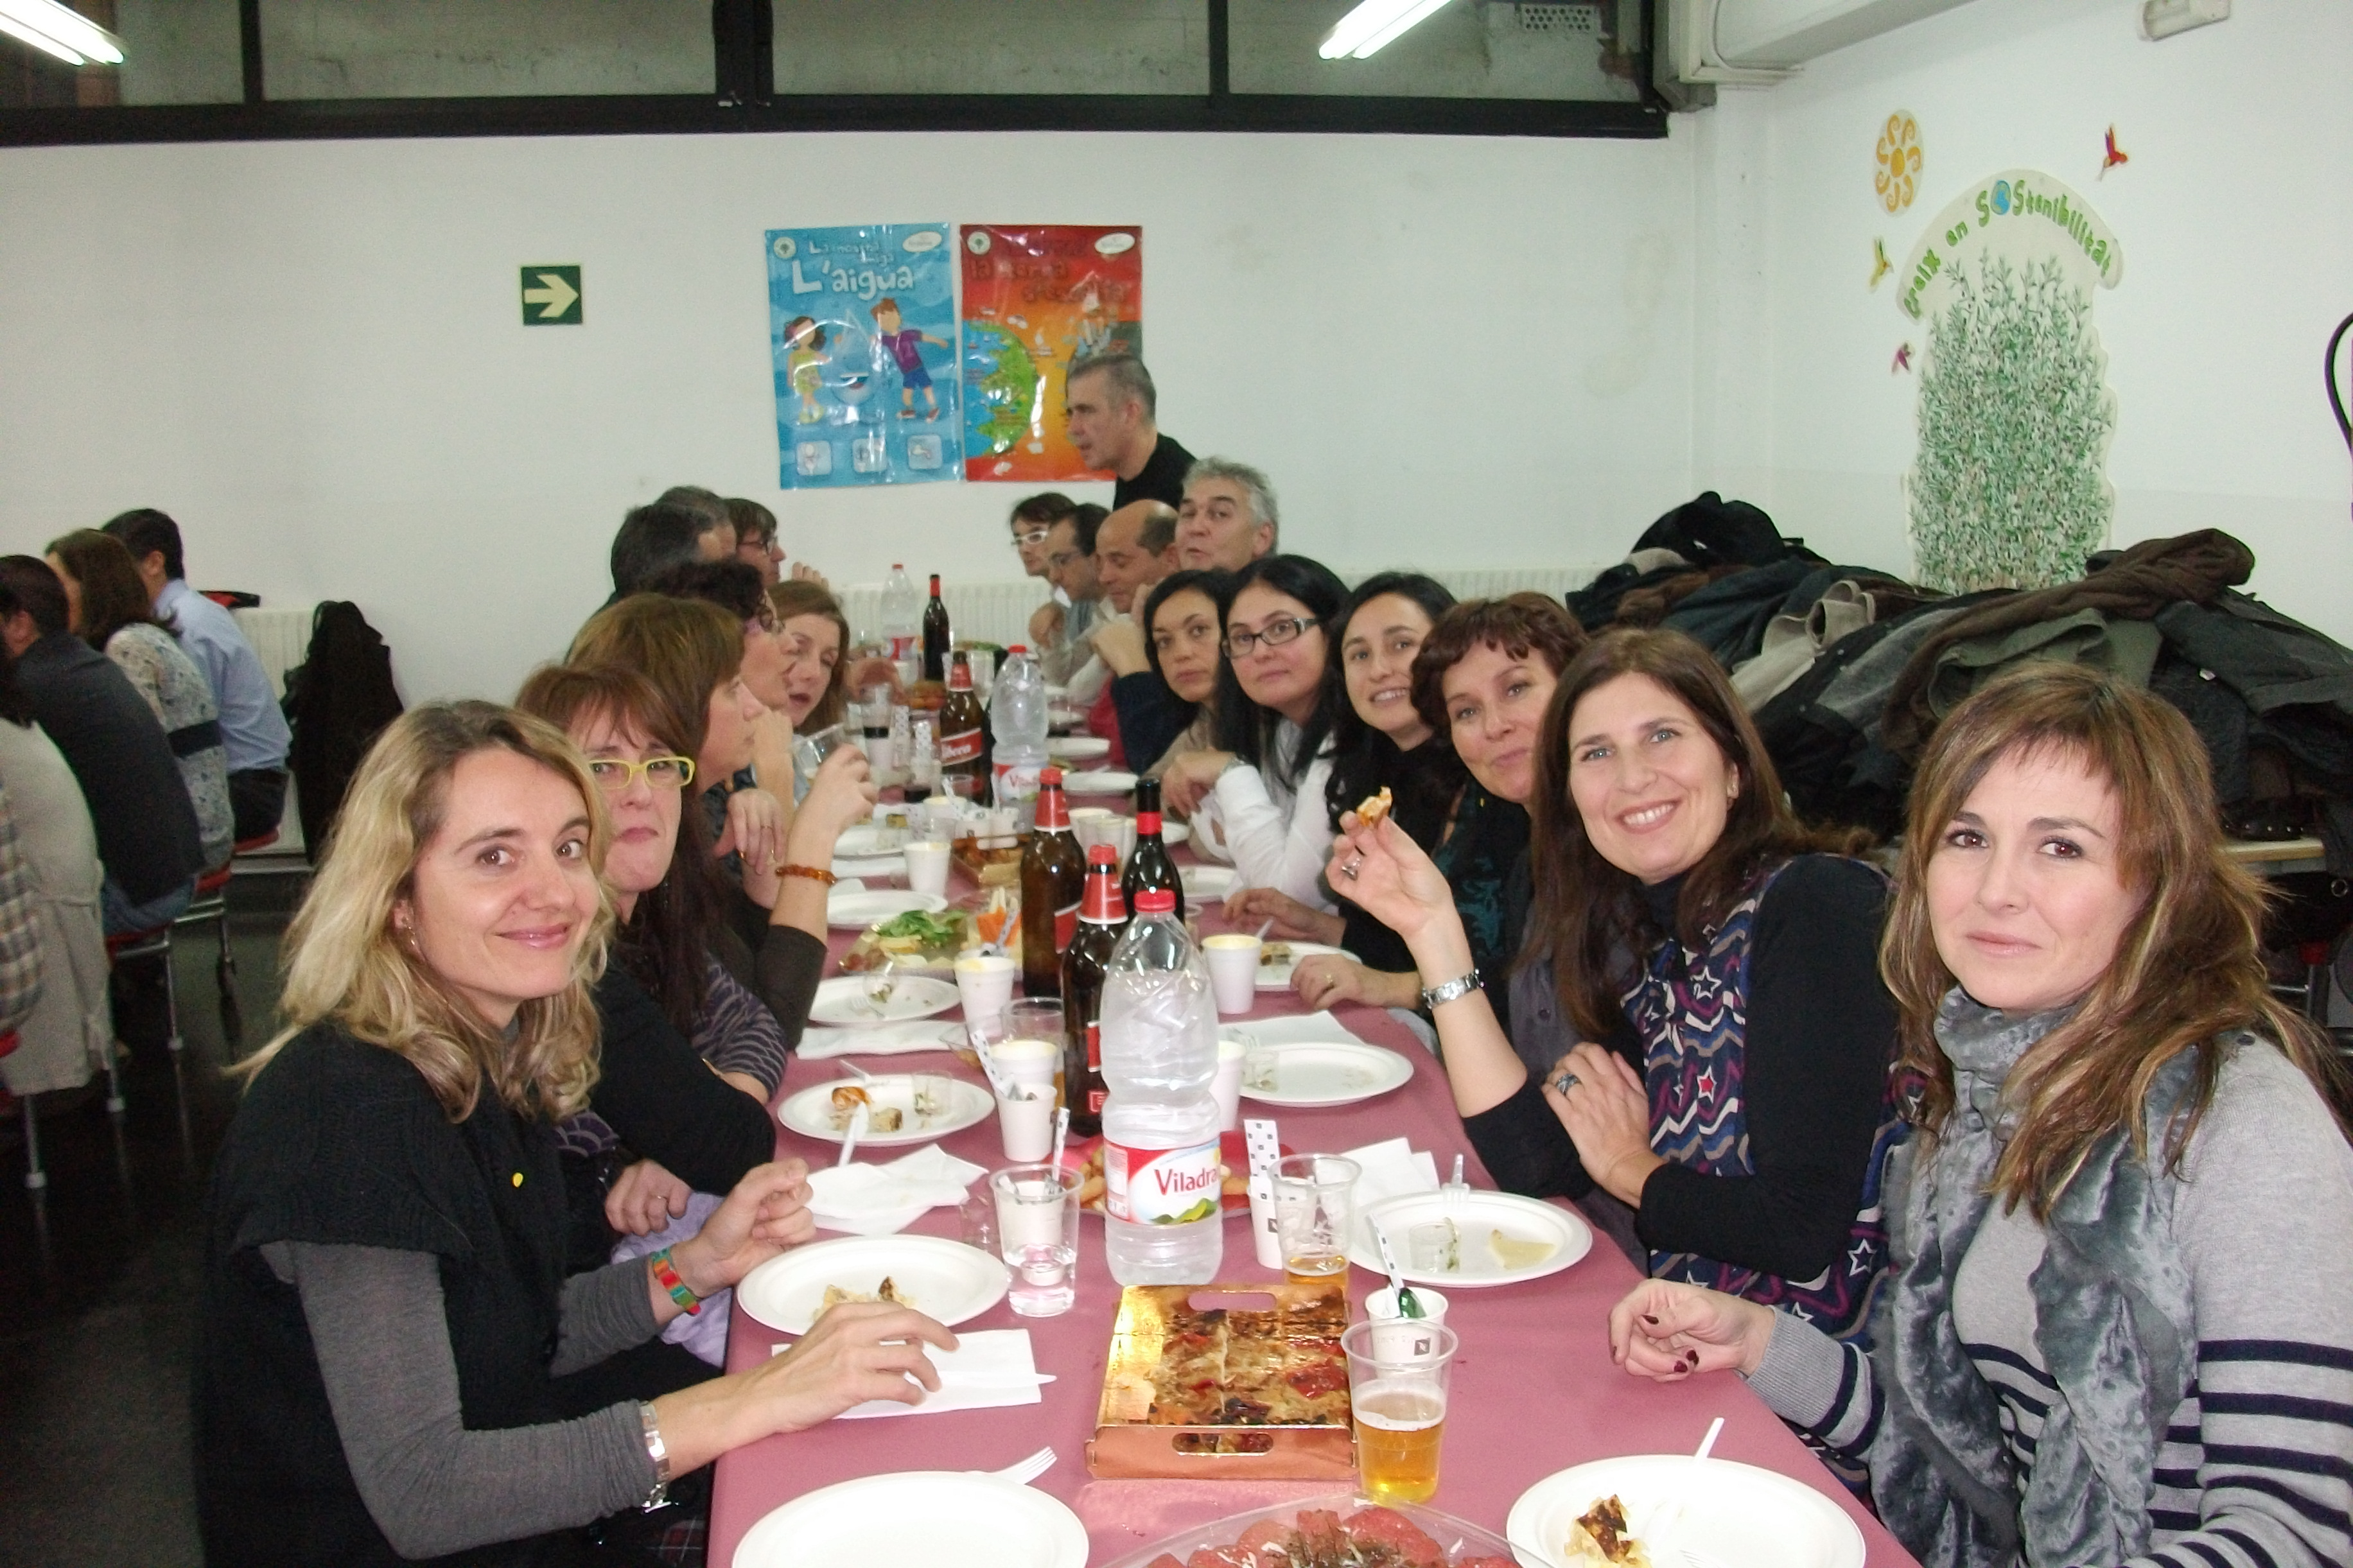
\includegraphics[width=9cm,keepaspectratio]{ampa/img/DSCF0920.JPG}


\end{news}
